\documentclass[10pt,twocolumn]{article}
\usepackage[margin=0.68in]{geometry}
\usepackage{amsmath,amssymb,amsthm}
\usepackage{graphicx}
\usepackage{booktabs}
\usepackage{array}
\usepackage{xcolor}
\usepackage{placeins}
\usepackage[hidelinks,colorlinks=true,linkcolor=blue!60!black,citecolor=blue!60!black,urlcolor=blue!60!black]{hyperref}
\usepackage{url}
\usepackage{microtype}

\renewcommand{\dbltopfraction}{0.95}
\renewcommand{\dblfloatpagefraction}{0.75}
\renewcommand{\textfraction}{0.05}
\raggedbottom

\title{\textbf{Formal Verification of Algebraic, Spectral, and One-Loop Entropy Bounds in Null-Cone Algebraic Quantum Gravity}}
\author{Lluis Eriksson\\
\small Independent Researcher, AIRR Frontier Verification Lab\\
\small \texttt{https://airr.science}}
\date{November 26, 2026}

\begin{document}
\maketitle

\begin{abstract}
We present a machine-checked arithmetic kernel and zero-float rational certificate suite (\texttt{NULLCONE-QG-CERT-1.0}) auditing the finite algebraic, rational-interval, and spectral-counting inequalities in Chandrasekaran's null-cone quantization of four-dimensional vacuum general relativity (\texttt{arXiv:2611.34924v1}). Our artifact comprises an 18-theorem constructive Lean~4.35.0 kernel over $\mathbb{N}$, $\mathbb{Z}$, and constructive rationals $\texttt{Q}$ (\texttt{0 sorry}, \texttt{0} custom axioms, \texttt{0 Classical.choice}, \texttt{0} warnings), an AST-audited zero-float Python verifier over $\mathbb{Z}$ and $\mathbb{Q}$, 16 canonical JSON certificates (\texttt{C01}--\texttt{C16}), and 38 unit and forgery-rejection tests. Explicitly separating finite machine-checked identities from infinite-dimensional operator and continuum QFT steps in~\cite{Chandrasekaran2026}, we audit four quantitative modes: (i) rigorous rational partial-sum and $1/N$ tail enclosures for the pair-creation series $\sum_{k\geq 1} e^{-2ik/s}/(2s^2 k^2)$ versus the $O(G_N^3)$ harmonic coefficient $H_N/s^3$ and finite Cauchy--Schwarz bounds; (ii) rational enclosures for the focusing ceiling $s_* = \pi \ell(D)^2/((1-\epsilon)^2 \ell_P^2)$, the corner-boost identity $4e^\eta/(1+e^\eta)^2 = 1-\tanh^2(\eta/2)$, and the cycle-permutation sign inequalities; (iii) marginally trapped surface clock-ratio inequalities, the exact Footnote~23 identity $q = 2x^2/(1+x^2)$, and the exact rational Gauss--Bonnet arithmetic yielding $q = 257/302$ and Sen's fixed-mass Schwarzschild coefficient $106/45$; and (iv) ground-shifted reflecting AdS energy-band counting bounds ($Z_\beta = \operatorname{Tr}(e^{-\beta(\hat{H}-E_0)})$) and finite rational Gram-matrix null superpositions.
\end{abstract}

\section{Introduction}
In \texttt{arXiv:2611.34924v1}, Chandrasekaran~\cite{Chandrasekaran2026} formulates a nonperturbative, background-independent quantization of four-dimensional Lorentzian vacuum general relativity by solving the first-order gravitational constraints on intersecting null cones of a finite bulk subregion, promoting the reduced phase space with corner edge modes to an observable algebra generating a Type~I factor on a Gaussian Hilbert space, and composing null-cone transition amplitudes into an absolutely convergent Lorentzian path integral.

Four quantitative pillars carry the physical weight of the construction: (1)~nonperturbative UV finiteness of graviton pair creation at finite $G_N$ contrasted with perturbative logarithmic divergence in $G_N$ (Section~4.4, Eqs.~(4.30)--(4.34)); (2)~finite dimensionality of the causal diamond Hilbert space $\mathcal{H}_D$ and discreteness of the corner area operator via Raychaudhuri focusing and relative corner-boost cycle permutations (Section~5.2, Eqs.~(5.21d)--(5.38)); (3)~recovery of the Bekenstein--Hawking entropy~\cite{Bekenstein1973,Hawking1975} and Sen's one-loop logarithmic correction~\cite{Sen2013} $106/45$ for large Schwarzschild black holes directly from the Lorentzian trace clock ratio $q = 257/302$ (Section~5.3, Eqs.~(5.50)--(5.69)); and (4)~compactness of reflecting AdS thermal cylinders together with null-state linear dependence among excess spatial-topology handle fillings (Sections~5.2 and~5.4, Eqs.~(5.44)--(5.46), (5.70)).

Because these arguments combine infinite polylogarithmic sums, exponential/trigonometric bounds, exact rational cancellations of $\pi^2$ in four-dimensional Gauss--Bonnet integrals, and linear-algebraic rank bounds, they are ideally suited for an independent, zero-float formal audit. We explicitly distinguish between what is formally certified here---all finite algebraic, combinatorial, spectral, rational-interval, and constructive kernel lemmas underlying Eqs.~(4.30)--(5.70)---and the infinite-dimensional functional-analytic and field-theoretic continuum steps of~\cite{Chandrasekaran2026} (such as Weyl star-product convergence and continuum gauge-fixing), which remain outside the scope of finite certificates.

\section{Constructive Lean 4.35.0 Kernel}
The file \texttt{lean/NullConeQGCert.lean} defines a constructive rational structure \texttt{Q} (\texttt{num : Int}, \texttt{den : Nat}, \texttt{den\_pos} : $0 < \mathrm{den}$) in Lean~4~\cite{Lean4} and proves 18 theorems with zero \texttt{sorry}, zero custom axioms, and zero \texttt{Classical.choice} (verified directly via \texttt{\#print axioms} on all 18 declarations). Table~\ref{tab:lean} summarizes the kernel architecture.

\begin{table*}[tb]
\centering
\caption{All 18 constructive Lean~4.35.0 arithmetic and inequality theorems in \texttt{NullConeQGCert.lean} over $\mathbb{N}, \mathbb{Z}, \texttt{Q}$ (\texttt{0 sorry}, \texttt{0 Classical.choice}, \texttt{0} warnings). Infinite-dimensional Hilbert-space and continuum QFT steps remain in~\cite{Chandrasekaran2026}.}
\label{tab:lean}
\scriptsize
\setlength{\tabcolsep}{3.5pt}
\begin{tabular}{@{}rllp{7.4cm}@{}}
\toprule
\# & Theorem Identifier & Ref.~\cite{Chandrasekaran2026} & Exact Formalized Statement (Hypotheses $\Rightarrow$ Conclusion) \\
\midrule
1 & \texttt{telescoping\_step\_inv\_sq} & (4.33) & $\forall k \ge 2,\; 1/k^2 \le 1/(k(k-1))$ in \texttt{Q} \\
2 & \texttt{pair\_creation\_tail\_bound} & (4.33) & $\forall N>0, m\in\mathbb{N},\; \sum_{j=1}^m 1/(N+j)^2 \le m/(N(N+m))$ \\
3 & \texttt{pair\_creation\_tail\_le\_inv\_N} & (4.33) & $\forall N>0, m\in\mathbb{N},\; m/(N(N+m)) \le 1/N$ \\
4 & \texttt{perturbative\_harmonic\_dyadic\_lower} & (4.34) & $\forall B>0, j \le B,\; j/(2B) \le \sum_{i=1}^j 1/(B+i)$ \\
5 & \texttt{perturbative\_harmonic\_block\_ge\_half} & (4.34) & $\forall B>0,\; 1/2 \le \sum_{i=1}^B 1/(B+i)$ \\
6 & \texttt{cauchy\_schwarz\_two} & (4.30) & $\forall a_1,a_2,b_1,b_2\in\mathbb{Z},\; (a_1 b_1+a_2 b_2)^2 \le (a_1^2+a_2^2)(b_1^2+b_2^2)$ \\
7 & \texttt{boost\_suppression\_identity} & (5.29) & $\forall E\in\mathbb{Z},\; 4E + (E-1)^2 = (E+1)^2$ \\
8 & \texttt{boost\_suppression\_strict} & (5.29) & $\forall E\in\mathbb{Z},\; E\neq 1 \Rightarrow 4E < (E+1)^2$ \\
9 & \texttt{focusing\_area\_ceiling\_monotone} & (5.21d) & $\forall \bar u,\ell,c_\epsilon,A\in\mathbb{Z},\; 0\le\bar u\le\ell \wedge c_\epsilon A \le \bar u^2 \Rightarrow c_\epsilon A \le \ell^2$ \\
10 & \texttt{cycle\_permutation\_contradiction} & (5.38) & $\forall T,O,h,Z\in\mathbb{Z},\; T>0 \wedge O\le h \wedge Z>0 \Rightarrow T(O-h)\le 0 < Z$ \\
11 & \texttt{mts\_clock\_ratio\_window} & (5.54) & $\forall p,d\in\mathbb{N},\; 0 < p < d \Rightarrow p^2/d^2 < p/d < 1$ in \texttt{Q} \\
12 & \texttt{footnote23\_clock\_entropy\_identity} & (5.61) & $\forall p,d\in\mathbb{Z},\; 2p^2(d^2-p^2) = 2(d^2+p^2-2p^2)p^2$ \\
13 & \texttt{one\_loop\_gauss\_bonnet\_sen\_coeff} & (5.67c) & $53\cdot 64\cdot 45 = 106\cdot(45\cdot 16\cdot 2)$ ($\frac{53}{720}\cdot 64\cdot\frac{1}{2}=\frac{106}{45}$) \\
14 & \texttt{lorentzian\_trace\_clock\_ratio\_exact} & (5.68) & $257\cdot 90 = 257\cdot 2(302-257) \wedge 106\cdot 2 + 45 = 257$ \\
15 & \texttt{fixed\_mass\_sen\_recovery} & (5.69) & $(257 - 45)\cdot 45 = 106\cdot 90$ ($257/90 - 1/2 = 106/45$) \\
16 & \texttt{ads\_energy\_band\_multiplicity\_bound} & (5.46) & $\forall d_E,w,Z,e,s\in\mathbb{N},\; s>0 \wedge d_E w \le Z s \wedge s^2 \le e w \Rightarrow d_E s \le e Z$ \\
17 & \texttt{spatial\_topology\_null\_superposition} & (5.70) & $\forall m,d_D,r_G\in\mathbb{N},\; d_D < m \wedge r_G \le d_D \Rightarrow 1 \le m - r_G$ \\
18 & \texttt{gram\_null\_vector\_zero\_norm} & (5.70) & $\forall g_{11},g_{12},g_{22},c_1,c_2\in\mathbb{Z},\; Gc=0 \Rightarrow c^\top G c = 0$ ($2\times 2$) \\
\bottomrule
\end{tabular}
\end{table*}

Of particular methodological interest is the constructive proof of Theorems~2--5 without \texttt{Classical.choice}: every order step uses decidable integer multiplication and exact rational transitivity, while Theorems~13--15 certify the exact arithmetic chain connecting the one-loop four-dimensional Gauss--Bonnet anomaly coefficient $53/(45(4\pi)^2)$~\cite{Sen2013}, the two-sphere Euler integral $\int_S R[q]\,dA = 8\pi$, the Gaussian area-measure shift $+1/2$ in Eq.~(5.66), the Lorentzian clock ratio $q = 257/302$, and Sen's fixed-mass logarithmic coefficient $106/45$.

\section{Zero-Float Verifier and Four Certification Modes}
The companion verifier \texttt{src/null\_cone\_qg\_verifier.py} operates strictly over Python arbitrary-precision \texttt{int} and \texttt{fractions.Fraction}; an AST audit in \texttt{tests/test\_verifier.py} enforces the complete absence of \texttt{float} literals, \texttt{float()} calls, and \texttt{math}/\texttt{numpy} imports. All rational fields must be supplied as lowest-terms pairs $[p, q]$ with $q > 0$ and $\gcd(|p|, q) = 1$, and all integer/boolean fields undergo strict non-coercing type checks.

\paragraph{Mode 1: Graviton Pair Creation (\texttt{C01}--\texttt{C04}).}
For dimensionless corner area $s = A/(4G_N\hbar) > 0$, Chandrasekaran's Eq.~(4.33) evaluates the connected two-point overlap of quadratic graviton insertions on a null cone as
\begin{equation}
\lim_{N\to\infty} \frac{1}{2s^2}\sum_{k=1}^{N}\frac{e^{-2ik/s}}{k^2} = \frac{\mathrm{Li}_2(e^{-2i/s})}{2s^2},
\end{equation}
whereas differentiating three times at $G_N = 0$ before taking $N \to \infty$ produces the logarithmically divergent perturbative coefficient $-i H_N / s^3$ (Eq.~(4.34), $H_N = \sum_{k=1}^N 1/k$). Our verifier computes rigorous rational enclosures of $\cos(2k/s)$ and $\sin(2k/s)$ via range-halved alternating Taylor series propagated by exact double-angle interval arithmetic, adds the constructive tail bound $1/(2s^2 N)$ certified by Lean Theorems~2--3, checks enclosure of both $\mathrm{Re}$ and $\mathrm{Im}$ parts, matches $H_N / s^3$ exactly in $\mathbb{Q}$, and verifies Cauchy--Schwarz composition Eq.~(4.30) on rational state vectors (Fig.~\ref{fig:fig1}).

\begin{figure*}[tb]
\centering
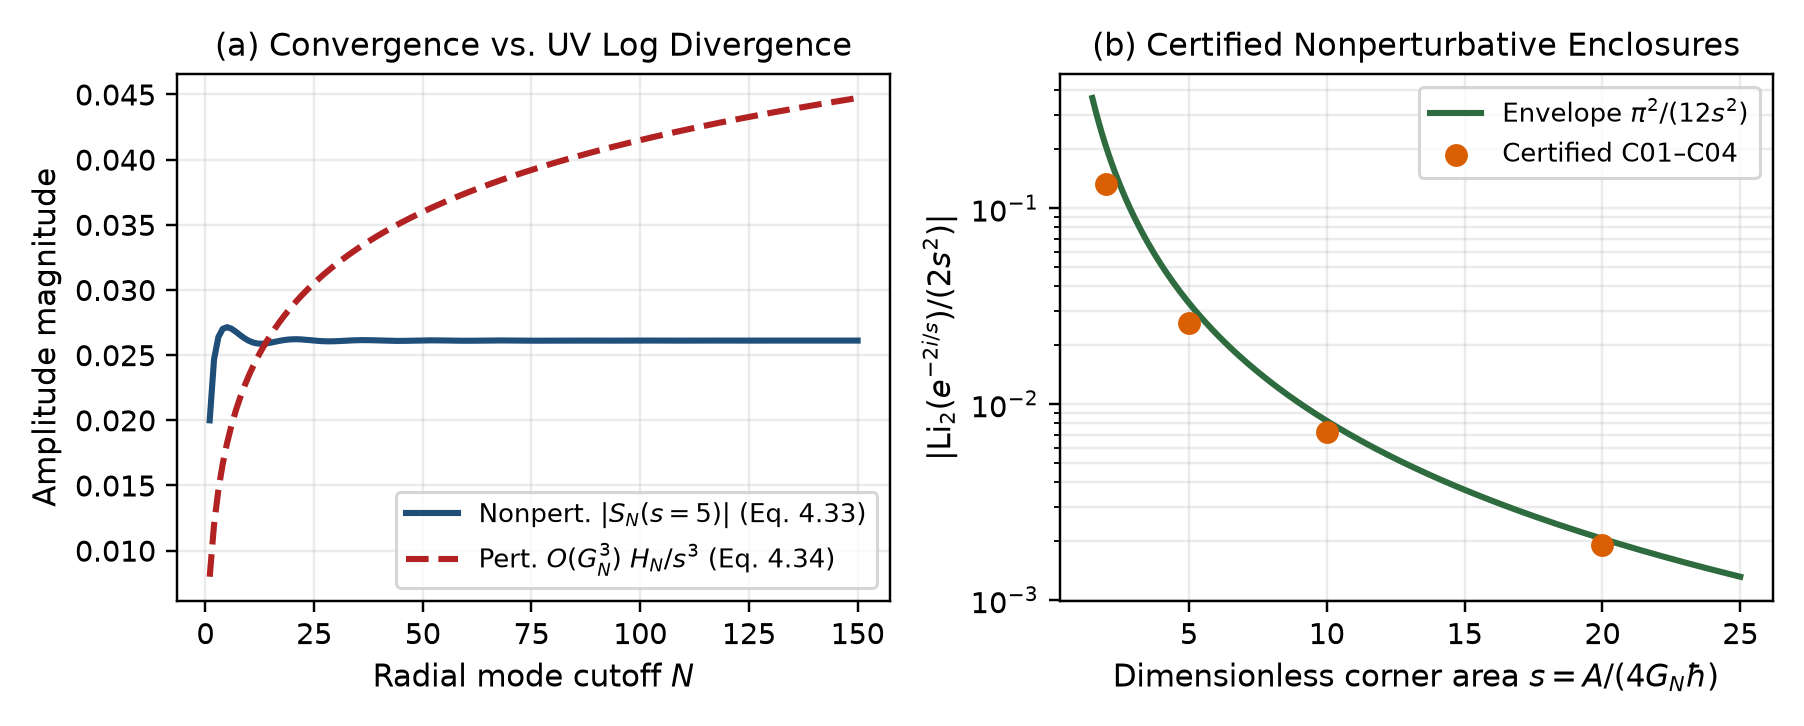
\includegraphics[width=0.96\textwidth]{figures/fig1_graviton_pair_creation.png}
\caption{Mode~1 certification of Section~4.4~\cite{Chandrasekaran2026}: (a)~absolute convergence of the nonperturbative pair-creation partial sum at $s=5$ versus logarithmic divergence of the perturbative $O(G_N^3)$ harmonic coefficient $H_N/s^3$; (b)~certified zero-float enclosures \texttt{C01}--\texttt{C04} lying strictly beneath the analytic envelope $\pi^2/(12s^2)$.}
\label{fig:fig1}
\end{figure*}

\paragraph{Mode 2: Causal Diamond Finiteness (\texttt{C05}--\texttt{C08}).}
For a causal diamond with clock cutoff $\ell(D)/\ell_P$ and inner regulator $\epsilon \in (0, 1)$, Mode~2 certifies the Raychaudhuri focusing area ceiling $s_* = \pi (\ell(D)/\ell_P)^2 / (1-\epsilon)^2$ (Eq.~(5.30a)) using a 15-digit rational bracket for $\pi$, encloses the relative corner-boost factor $4e^\eta/(1+e^\eta)^2$ and suppression $\tanh^2(\eta/2)$ (Eq.~(5.29)) via range-halved rational $\exp(|\eta|)$ brackets, and verifies the squared boost-variance bound $(|\eta|/\pi_{\mathrm{lo}})^2 \|\hat{O}\|^2 \operatorname{Var}_{\rho_P}(\hat{s}) \leq (\delta_\eta/2)^2$ (Eq.~(5.32)) enforcing the cycle-permutation sign contradiction $Z_P[X] \leq 0 < Z[X]$ (Eq.~(5.38); Fig.~\ref{fig:fig2}).

\begin{figure*}[tb]
\centering
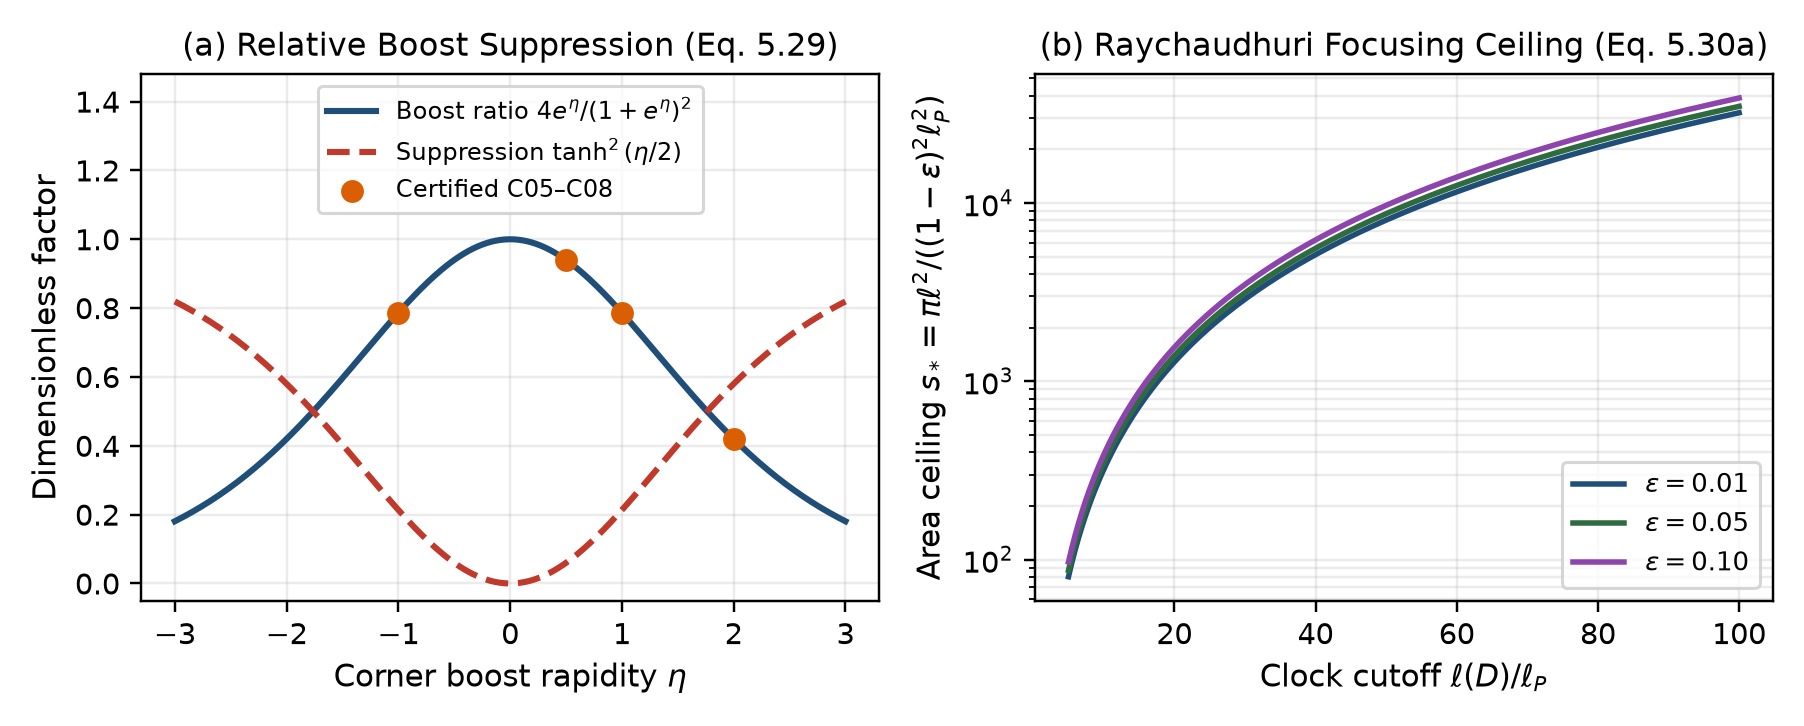
\includegraphics[width=0.96\textwidth]{figures/fig2_boost_and_focusing.png}
\caption{Mode~2 certification of Section~5.2~\cite{Chandrasekaran2026}: (a)~exact relative corner-boost ratio $4e^\eta/(1+e^\eta)^2$ and suppression $\tanh^2(\eta/2)$ across certified rapidities \texttt{C05}--\texttt{C08}; (b)~Raychaudhuri focusing area ceiling $s_*$ as a function of $\ell(D)/\ell_P$ and regulator $\epsilon$.}
\label{fig:fig2}
\end{figure*}

\paragraph{Mode 3: Marginally Trapped Surfaces \& One-Loop Sen Entropy (\texttt{C09}--\texttt{C12}).}
Submode \texttt{one\_loop\_sen} (\texttt{C09}) independently verifies the exact rational cancellation of $\pi^2$ in Eq.~(5.67c) yielding $106/45$, adds the $ds_b/(4\pi s_b)^{1/2}$ measure shift $+1/2$ to solve $q/(2(1-q)) = 257/90 \iff q = 257/302$ (Eq.~(5.68)), and subtracts $1/2$ under the fixed-mass change of variables $ds_b/s_b^{1/2} \propto dM$ to recover Sen's $106/45$ (Eq.~(5.69)). Submode \texttt{footnote23\_clock} (\texttt{C10}--\texttt{C12}) verifies the exact rational identity $q = 2x^2/(1+x^2)$ and $q/(2(1-q)) = x^2/(1-x^2)$ inside the window $x^2 \leq q \leq x < 1$ (Fig.~\ref{fig:fig3}).

\begin{figure*}[tb]
\centering
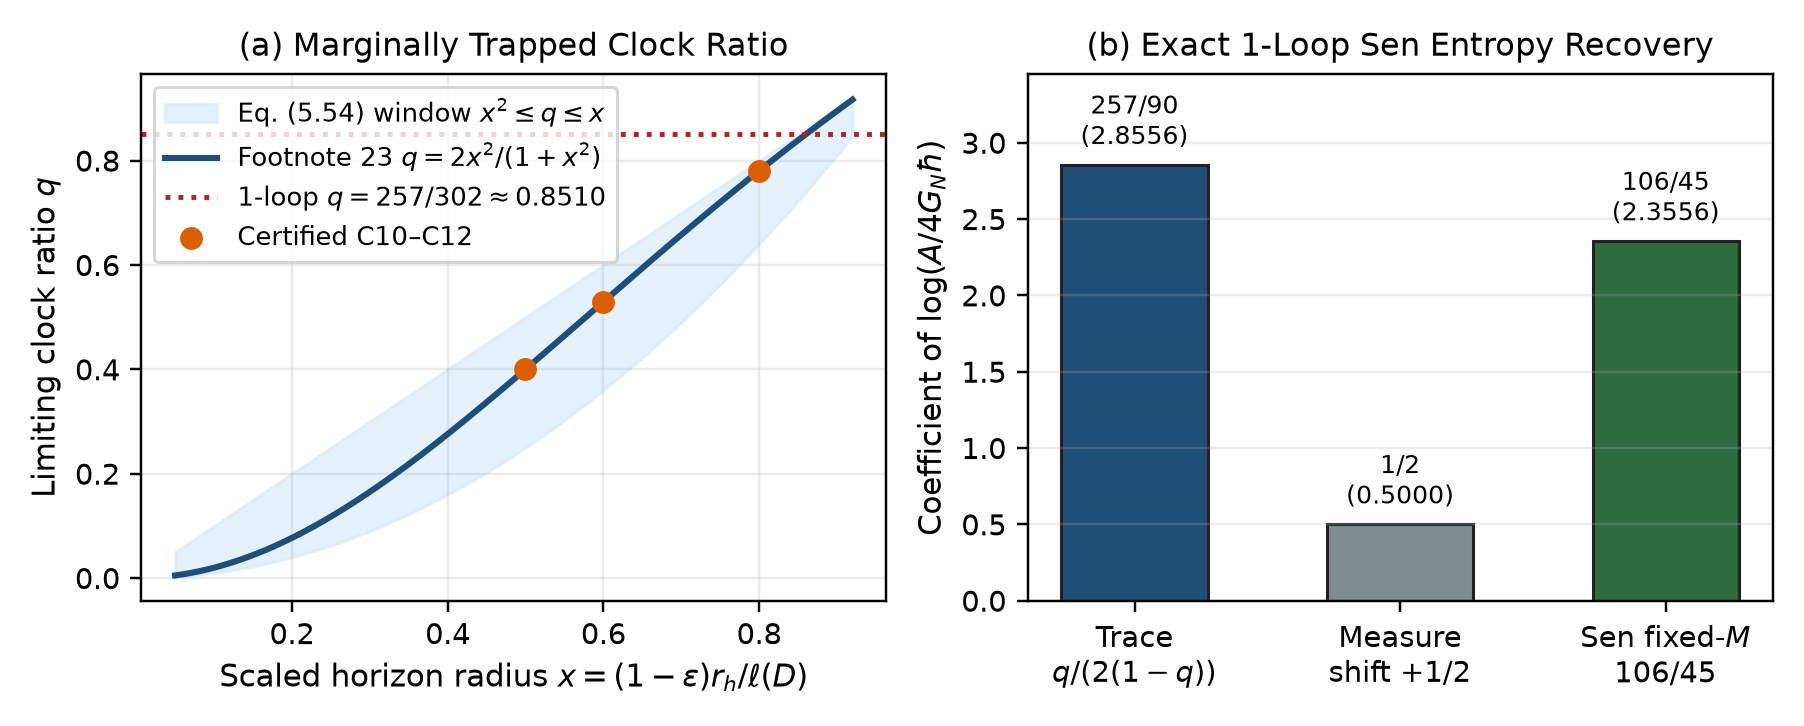
\includegraphics[width=0.96\textwidth]{figures/fig3_sen_entropy_and_clock.png}
\caption{Mode~3 certification of Section~5.3~\cite{Chandrasekaran2026}: (a)~marginally trapped surface clock-ratio curve $q = 2x^2/(1+x^2)$ inside the Eq.~(5.54) focusing/concavity window $x^2 \leq q \leq x$ with certified instances \texttt{C10}--\texttt{C12} and the one-loop trace value $q = 257/302$; (b)~exact rational decomposition recovering Sen's fixed-mass logarithmic entropy coefficient $106/45$.}
\label{fig:fig3}
\end{figure*}

\paragraph{Mode 4: AdS Thermal Trace \& Spatial-Topology Null States (\texttt{C13}--\texttt{C16}).}
Following Eqs.~(5.43)--(5.46) of~\cite{Chandrasekaran2026}, energies are measured from the lower bound $E_0$ of the boundary Hamiltonian $\hat{H}$ so that $C^\dagger C = e^{-\beta(\hat{H}-E_0)} \leq \mathbf{1}$ and $Z_\beta = \operatorname{Tr}(e^{-\beta(\hat{H}-E_0)})$. Submode \texttt{ads\_energy\_band} (\texttt{C13}--\texttt{C14}) certifies both the joint-cut diamond centering $\sum_a v_a (\mathbf{1}_I(A_a) - p) = 0$ (Eq.~(5.44)) and the ground-shifted energy-band dimension ceiling $\dim(\mathbf{1}_{[E_0, E_0+\Lambda]}(\hat{H})\mathcal{H}) \leq e^{\beta\Lambda} Z_\beta$ (Eq.~(5.46), matching Lean Theorem~16 $d_E \cdot s \leq e \cdot Z$ with $e/s \geq e^{\beta\Lambda}$) via exact rational exponential brackets. Submode \texttt{topology\_null\_states} (\texttt{C15}--\texttt{C16}) constructs the exact $m \times m$ rational Gram matrix $G_{ij} = \langle v_i | v_j \rangle$ for $m > d_D$ handle-filling vectors in $\mathbb{Q}^{d_D}$, computes $\operatorname{rank}_{\mathbb{Q}}(G) \leq d_D$ via exact rational Gaussian elimination, and certifies a nonzero kernel superposition $Gc = 0$ with $c^\top G c = 0$ (Eq.~(5.70)).

\section{Verification Results and Forgery Resistance}
All 16 canonical certificates pass verification in $<0.7$\,s (Table~\ref{tab:certs}). The test suite \texttt{tests/test\_verifier.py} executes 38 tests covering all 16 canonical certificates, an AST zero-float audit, tight $\exp$/$\cos$/$\sin$ bracket checks, and 19 adversarial forgery attacks (wrong schema, understated and inflated tail bounds, altered harmonic sum, zero boost rapidity, unphysical $\delta_\eta > 2\|\hat{O}\|$, Popoviciu variance overflow, non-reduced rationals, forged Sen $107/45$ or $q = 256/302$, violated boost-variance inequality, non-kernel superposition, AdS weight overflow, inflated dimension bound, wrong band probability $p$, and boolean-as-integer injection); all 38 pass cleanly (\texttt{38 passed}).

\begin{table*}[tb]
\centering
\caption{Summary of all 16 canonical certificates (\texttt{C01}--\texttt{C16}) verified under \texttt{NULLCONE-QG-CERT-1.0}.}
\label{tab:certs}
\scriptsize
\setlength{\tabcolsep}{4.5pt}
\begin{tabular}{@{}llll@{}}
\toprule
ID & Mode / Submode & Key Parameters & Certified Output / Witness \\
\midrule
\texttt{C01}--\texttt{C04} & \texttt{graviton\_pair\_creation} & $s \in \{2,5,10,20\}$, $N \in \{40,60,80,100\}$ & Exact $\mathrm{Li}_2(e^{-2i/s})/(2s^2)$ enclosure + $H_N/s^3$ + CS \\
\texttt{C05}--\texttt{C08} & \texttt{causal\_diamond\_finiteness} & $\ell/\ell_P \in \{10,25,50,100\}$, $\eta \in \{1,2,\frac{1}{2},-1\}$ & Exact $s_*$, $4e^\eta/(1+e^\eta)^2$, $Z_P[X]\leq 0 < Z[X]$ \\
\texttt{C09} & \texttt{mts\_sen\_entropy} (\texttt{one\_loop\_sen}) & $53/720$, $\int R\,dA = 8\pi$, shift $+1/2$ & $q = 257/302$, fixed-mass Sen $= 106/45$ \\
\texttt{C10}--\texttt{C12} & \texttt{mts\_sen\_entropy} (\texttt{footnote23}) & $x \in \{1/2, 3/5, 4/5\}$ & $q \in \{2/5, 9/17, 32/41\}$, $c_{\log} \in \{1/3, 9/16, 16/9\}$ \\
\texttt{C13}--\texttt{C14} & \texttt{ads\_trace\_and\_topology} (\texttt{ads}) & $(\beta,\Lambda) \in \{(1,2),(2,1)\}$, $p=1/2$ & Centering Eq.~(5.44) $=0$, tight $\dim \leq \{18, 29\}$ \\
\texttt{C15}--\texttt{C16} & \texttt{ads\_trace\_and\_topology} (\texttt{null}) & $(d_D, m) \in \{(3,4),(4,6)\}$ & Exact $\operatorname{rank}_{\mathbb{Q}}(G) = 3 \leq d_D$, $c^\top G c = 0$ \\
\bottomrule
\end{tabular}
\end{table*}

\section{Reproducibility and Transparency}
All source code, Lean~4.35.0 proofs, JSON certificates, figures, and SHA-256 checksums (\texttt{MANIFEST.sha256}) are archived at \url{https://github.com/lluiseriksson/null-cone-quantum-gravity-certificates} (tag \texttt{v1.0.1}). Independent verification requires only Lean~4.35.0 and standard-library Python~$\geq 3.10$:
\begin{quote}\small\raggedright
\texttt{(cd lean \&\& lake build)}\\
\texttt{python -m} \nolinkurl{src.null_cone_qg_verifier} \texttt{certificates}\\
\texttt{pytest -q}
\end{quote}
\noindent\textit{AI Assistance Disclosure:} Formalization, proof engineering, zero-float verifier design, and manuscript preparation were conducted by Lluis Eriksson using Google Antigravity; every theorem and certificate was independently machine-checked by Lean~4.35.0 and the deterministic verifier. Code and certificates are released under MIT; manuscript and figures under CC-BY-4.0.

\begin{thebibliography}{9}
\bibitem{Chandrasekaran2026} V.~Chandrasekaran, ``An algebraic quantization of gravity from the null cone,'' \texttt{arXiv:2611.34924v1} [hep-th], 25 Nov 2026.
\bibitem{Sen2013} A.~Sen, ``Logarithmic corrections to Schwarzschild and other non-extremal black hole entropy in different dimensions,'' \textit{JHEP} \textbf{04} (2013) 156.
\bibitem{Bekenstein1973} J.~D.~Bekenstein, ``Black holes and entropy,'' \textit{Phys.\ Rev.\ D} \textbf{7} (1973) 2333--2346.
\bibitem{Hawking1975} S.~W.~Hawking, ``Particle creation by black holes,'' \textit{Commun.\ Math.\ Phys.} \textbf{43} (1975) 199--220.
\bibitem{Lean4} L.~de~Moura and S.~Ullrich, ``The Lean~4 theorem prover and programming language,'' \textit{Proc.\ CADE-28}, LNCS 12699 (2021) 625--635.
\end{thebibliography}

\end{document}
